The separately frozen scalar experiment uses 4,096 paths under each of two laws, 65,536 evaluated observations and 32 training observations. It fixes $\gamma=\sigma=1$, $L=.5$, $r=0$, and public bounds $M_2=1$, $M_4=6$. The alternative is the iid Gaussian law of Theorem~\ref{thm:vanishing}; the boundary null is \eqref{eq:vanishing-null}. All four rules see the same return path within each law. The linear and two fixed Catoni stakes are $\gamma/2$; the original uniform-bound past-mean stake updates every 252 observations. No positive minimum-effect filter is applied.

\begin{table}[H]\centering\small

\begin{tabular}{lrrrr}\toprule

& \multicolumn{2}{c}{Crossings / 4096} & \multicolumn{2}{c}{Alternative final log capital} \\

Rule & Alternative & Null & Mean & MC SE \\\midrule

Linear cash-PARK & 3 & 0 & 0.97564 & 0.01307 \\

Catoni, geometry, fixed & 1 & 0 & 0.77040 & 0.01519 \\

Catoni, uniform, fixed & 0 & 0 & -5322.34919 & 0.00782 \\

Catoni, uniform, past mean & 0 & 0 & -0.00193 & 0.00006 \\

\bottomrule\end{tabular}

\caption{Controlled scalar cash-PARK diagnostic at individual level 5\%. Crossings are over all evaluated dates, not just the last date. The 252-date review counts happen to coincide with these counts at this horizon. These are statistical paths, not financial market replications.}\label{tab:vanishing}\end{table}

A subsequent summary of the same saved paths gives mean realized cumulative cash advantage $J_n=3.87129$ (MC SE 0.01583); 14 of 4,096 realized sums are negative. This is a post-hoc fixed-horizon description, not another experiment, a stopped-cost estimate or a verification of the almost-sure limit.

The linear crossing fraction is 0.000732 (Wilson 95\% interval [0.000249, 0.002151]); the geometric fraction is 0.000244 ([0.000043, 0.001382]). Three versus one crossing does not establish a finite-sample power ranking. All rules have zero observed alternative crossings at the separately declared 1\% and .1\% levels. Every null count is zero at all three levels; the Wilson 95\% upper bound for each zero count is .000937. Zero observed crossings do not establish zero probability.

The mean integrated squared target is 7.70966, and the mean cumulative conditional cash benefit is 3.85483 in the toy utility units. These are unstopped-horizon means, not expected benefits at rejection or calibrated financial returns. The mean evaluator log likelihood ratio is 0.97827; the linear rule has mean absolute log discrepancy 0.03746. The finite-horizon diagnostics do not establish the asymptotic bounds by themselves.

Independent replay checks 39,888 scalar checkpoint values using direct multiplication of factors and separate Gaussian density calculations. It covers a fixed prefix of 8 paths per law, not all simulated paths; the maximum absolute discrepancy is 8.37e-11. All declared paths and failed-to-cross outcomes are retained. No horizon, bound, bet or seed was retuned after observing low power.

\begin{figure}[H]\centering

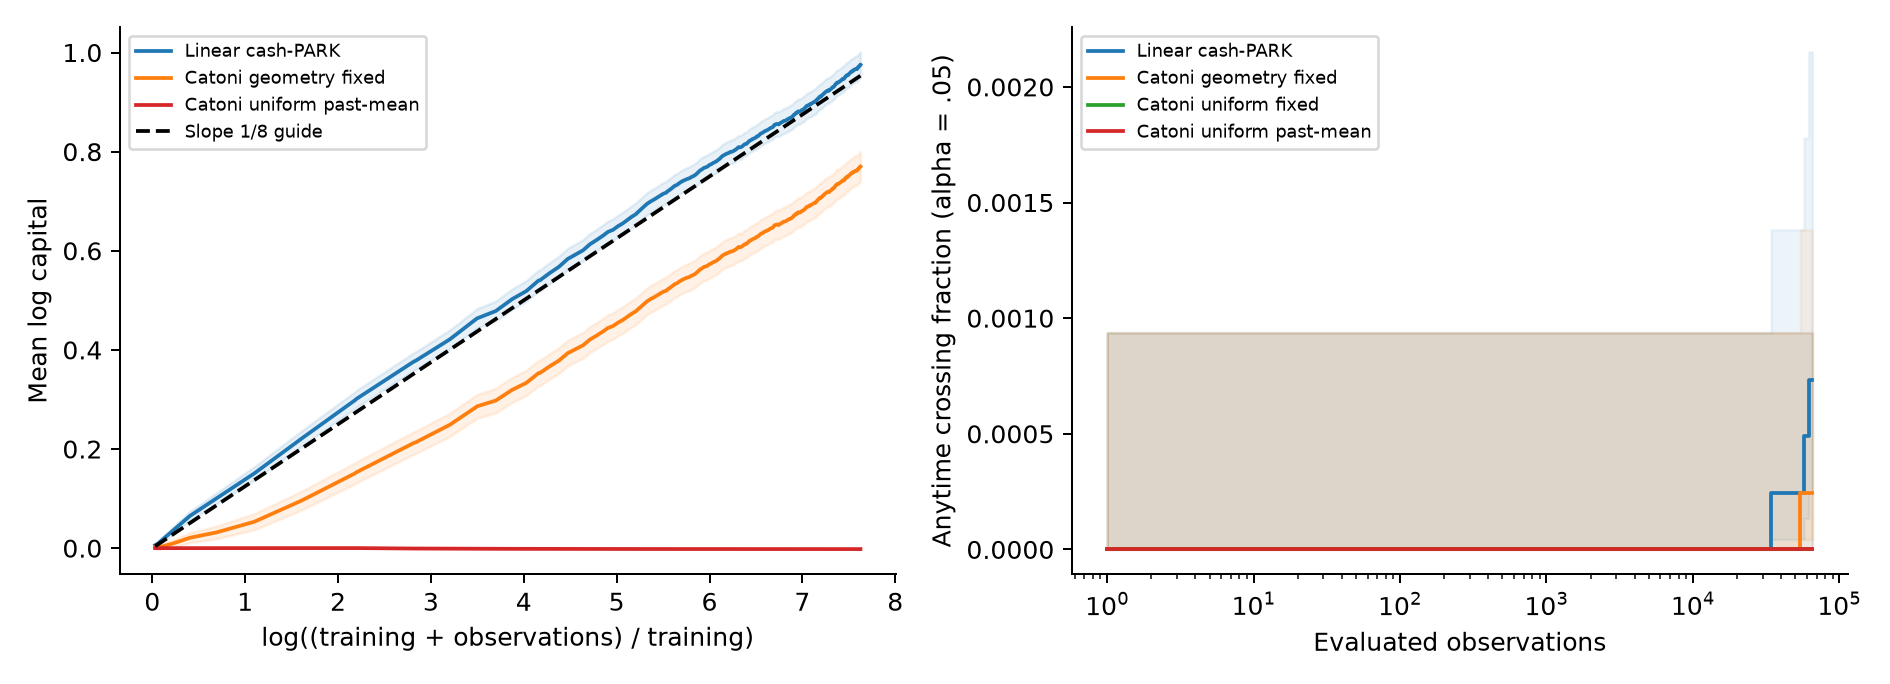
\includegraphics[width=\linewidth]{figures/vanishing_gain.png}

\caption{Scalar vanishing-gain diagnostic. Left: mean log capital with pointwise 95\% Monte Carlo intervals; the uniform fixed-bet rule is omitted from this panel because its large negative values obscure the other series. The $1/8$ line is a slope guide, not an exact finite-horizon formula. Right: all-date crossing fractions at level 5\% with pointwise Wilson intervals. Bands are not simultaneous over time.}\label{fig:vanishing}\end{figure}

Eventual crossing and a sharp confidence exponent can coexist with very low finite-horizon power. The experiment supplies no financial performance improvement or adaptation theorem for changing regimes.
